\documentclass[10pt,twocolumn,letterpaper]{article}

\usepackage{cvpr}
\usepackage{times}
\usepackage{epsfig}
\usepackage{graphicx}
\usepackage{amsmath}
\usepackage{amssymb}
\usepackage{xcolor}
\usepackage{soul}
\usepackage{booktabs}
\usepackage{float}
\usepackage{caption}
\captionsetup[table]{skip=5pt}
\usepackage{tabularx} % for 'tabularx' environment
\usepackage{adjustbox}

\usepackage{tikz}
\usepackage{pgfplots}
\usepackage{subcaption}
\pgfplotsset{scaled y ticks=false}

\definecolor{mygreen}{RGB}{22, 168, 58}
\definecolor{myorange}{RGB}{255, 118, 33}
\definecolor{myblue}{RGB}{10, 143, 209}
\definecolor{myred}{RGB}{235, 21, 21}

\pgfplotsset{compat=1.12}



\pgfplotsset{
  every axis plot/.append style={line width=1.0pt},
  every axis plot post/.append style={
    every mark/.append style={line width=1.6pt,draw=green,fill=red}
  },
  xticklabel style={
        /pgf/number format/fixed,
        /pgf/number format/precision=5
  },
  scaled x ticks=false,
  scaled y ticks=false,
  width= 1.00\columnwidth
}

\newcommand{\RBF}{myblue}
\newcommand{\Ptwo}{myorange}
\newcommand{\Pthree}{myred}
\newcommand{\VSV}{mygreen}
\newcommand{\legendentries}{\addlegendentry{Standard RBF} \addlegendentry{Pooling ($2 \times 2$)} \addlegendentry{Pooling ($3 \times 3$)} \addlegendentry{VSV SVM}}




% Include other packages here, before hyperref.

% If you comment hyperref and then uncomment it, you should delete
% egpaper.aux before re-running latex.  (Or just hit 'q' on the first latex
% run, let it finish, and you should be clear).
\usepackage[breaklinks=true,bookmarks=false]{hyperref}

\cvprfinalcopy % *** Uncomment this line for the final submission

\def\cvprPaperID{****} % *** Enter the CVPR Paper ID here
\def\httilde{\mbox{\tt\raisebox{-.5ex}{\symbol{126}}}}

% Pages are numbered in submission mode, and unnumbered in camera-ready
%\ifcvprfinal\pagestyle{empty}\fi
%\setcounter{page}{4321}
\begin{document}

%%%%%%%%% TITLE
\title{Incorporating Invariances in Support Vector Machines using Max-Pooling Kernels}

\author{Tuhin Das\\
Delft University of Technology\\
%Institution1 address\\
{\tt\small t.das@student.tudelft.nl}
% For a paper whose authors are all at the same institution,
% omit the following lines up until the closing ``}''.
% Additional authors and addresses can be added with ``\and'',
% just like the second author.
% To save space, use either the email address or home page, not both
}

\maketitle
%\thispagestyle{empty}

%%%%%%%%% ABSTRACT
\begin{abstract}
\color{lightgray}
   Lorem ipsum dolor sit amet, consectetur adipiscing elit, sed do eiusmod tempor incididunt ut labore et dolore magna aliqua. Ut enim ad minim veniam, quis nostrud exercitation ullamco laboris nisi ut aliquip ex ea commodo consequat. Duis aute irure dolor in reprehenderit in voluptate velit esse cillum dolore eu fugiat nulla pariatur.
\end{abstract}

%%%%%%%%% BODY TEXT


\section{Introduction}

For certain tasks like digit recognition, image classifiers often benefit from invariances to image translations and rotations, as object appearance is usually more important than object location. 
Some classifiers such as the Convolutional Neural Network (CNN) are invariant to small image transformations to some extent \cite{albawiUnderstandingConvolutionalNeural2017}. 
Many classifiers are however not invariant, an example of which is the Support Vector Machine (SVM). 
The classification capabilities of Support Vector Machine can be improved by incorporating invariances to image transformation. 

Various methods exist to incorporate invariances in SVMs \cite{lauerIncorporatingPriorKnowledge2008}, but many methods either rely on data augmentation or manually defining which transformations a SVM should become invariant to.  
In this paper we present a new method to make SVMs more invariant, where data augmentation and manually defining transformations are not necessary. 
Inspired by CNNs, which are partially invariant due to their max-pooling filters \cite{goodfellowDeepLearning2016, hutchisonEvaluationPoolingOperations2010b}, we attempt to incorporate max-pooling filters in SVMs. 
We modify Radial Basis Function (RBF) kernels of SVMs to use max-pooling filters, such that the kernels become invariant to image transformations.
The kernels should denote more similarities between different samples of a similar class, even though the images are translated or rotated compared to each other.  


We make the following contributions.
First we show that max-pooling filters can be incorporated in Gaussian RBF kernels to incorporate invariances.
Second, we remove the need to manually define which image transformations the SVM should be invariant against, which is needed in certain methods \cite{decosteTrainingInvariantSupport2002, scholkopfIncorporatingInvariancesSupport1996}.
Third, we show that the use of max-pooling kernels can make SVMs more robust against noise in the data samples. 






%------------------------------------------------------------------------
\section{Related Work}

Invariance of the class to a transformation in the input is a type of prior knowledge that can be incorporated in a classifier \cite{lauerIncorporatingPriorKnowledge2008}. 
An effective method to incorporate invariances in a classifier is to augment the data with transformed versions of training samples.
Data augmentation has been shown to be effective in CNNs using data sets with geometrically transformed training samples \cite{kauderer-abramsQuantifyingTranslationInvarianceConvolutional2017} and with photometrically transformed samples \cite{taylorImprovingDeepLearning2017}. 

The Virtual Support Vector (VSV) method \cite{scholkopfIncorporatingInvariancesSupport1996} is a method based on data augmentation, specifically for SVMs. 
Instead of augmenting the original data set, a SVM is first trained using the original data set. 
Afterwards a new training set is generated by applying transformations on the support vectors of the trained SVM. 
A new SVM is trained on the transformed support vector set, which makes the second SVM more invariant against the transformations. 
The downside of data augmentation techniques is that the training duration becomes larger. 
Further, it is necessary to manually define which transformations are used to augment the data set.

Instead of augmenting data sets, some methods modify SVM kernels to induce invariances while learning. 
Examples of such kernel methods are jittering kernels \cite{decosteTrainingInvariantSupport2002}, tangent distance kernels \cite{haasdonkTangentDistanceKernels2002} and Haar-integration kernels \cite{haasdonkInvarianceKernelMethods2005}. 
Jittering kernels for example consider the transformed variations of its input samples given a set of manually defined transformations. 
Jittering kernels define the distance between two samples $\textbf{x}_i$ and $\textbf{x}_j$ as the shortest distance between $\textbf{x}_i$ and each transformed variation of $\textbf{x}_j$. 
A benefit of such kernel methods is that the data set does not need to be enlarged.
To keep this benefit we also show a method for incorporating invariances by modifying kernels only.  

%Instead of augmenting data sets, it is possible to consider transformed variations of data samples in so called jittering kernels for SVMs \cite{decosteTrainingInvariantSupport2002}.
%Given two input samples $\textbf{x}_i$ and $\textbf{x}_j$, jittering kernels perform all predefined transformations on $\textbf{x}_i$ to find a transformed sample closest to $\textbf{x}_j$. 
%Jittering kernels thus define a notion of similarity between samples, while taking the predefined transformations into account. 
%











\begin{figure*}[t]
\begin{center}
\includegraphics[width=1.0\textwidth]{images/max-pooling}
\end{center}
\caption{Two steps are shown of a $4\times 4$ input layer that is filtered with a max-pooling filter of size $2\times 2$ with a stride of 1. Each square of $2\times 2$ in the original layer is merged into a single value in the output layer by taking the maximum value in the $2\times 2 $ filter. The resulting output layer has a reduced size of $3\times 3$.}
\label{max-pooling}
\end{figure*}


%-------------------------------------------------------------------------


\section{Max-Pooling}

Max-pooling is a process where an input representation is downsampled by taking the maximum of groups of input values. 
Max-pooling can be used to reduce the dimensionality of layer vectors to create a downsampled vector that retains the most important information. 
For example, CNNs use max-pooling to retain the presence of signals in input representations rather than the exact location of the signals. 

Max-pooling is applied by using a filter of a predefined size $m \times n$ and by sliding this filter across a rectangular input representation such as an image.
The output of the filter is the maximum of the $mn$ values covered by the filter. 
The filter can be shifted one position at a time or can jump across the input layer with a predefined stride size.
By applying this filter on a complete input layer, the input is effectively downsampled into a new layer with less features. 
Fig. \ref{max-pooling} shows the working of a max-pooling filter of size $2\times 2$ with a stride of 1 on a $4\times 4$ input layer.



%-------------------------------------------------------------------------




\section{Max-Pooling Kernels}

Support Vector Machines \cite{vapnikNatureStatisticalLearning1995} make use of various kernels to train on the data set and to predict labels using its support vectors. 
Several kernel functions are available such as the linear kernel, polynomial kernel and the Gaussian RBF kernel, which are respectively defined as

\begin{align}
	k_{\text{linear}}(\textbf{x}_i, \textbf{x}_j) & = \langle \textbf{x}_i, \textbf{x}_j\rangle\\
	k_{\text{poly}}(\textbf{x}_i, \textbf{x}_j) & = \langle (\textbf{x}_i, \textbf{x}_j\rangle + 1)^d, \enspace d\in \mathbb{N}\\
	k_{\text{RBF}}(\textbf{x}_i, \textbf{x}_j) & = \exp \bigg(- \frac{\| \textbf{x}_i - \textbf{x}_j \|^2}{2\sigma ^2}\bigg), \enspace \sigma > 0,
\end{align}


\noindent where $\textbf{x}_i$ and $\textbf{x}_j$ are two input samples, $d$ is the polynomial degree and $\sigma$ is a free parameter. Often $\gamma = 2\sigma^{-2}$ is used as the free parameter. 
\noindent Because the kernels define the notion of similarity for a SVM, the kernel choice will influence the performance of a SVM. 
It is necessary to choose a fitting kernel for any given problem to achieve optimal SVM performance.
In order to incorporate a max-pooling filter in a kernel, this must be possible regardless of the type of kernel. 

To create a max-pooling kernel, we incorporate a max-pooling filter in any given kernel $k$ as follows.
First, we define a function $p$ that takes a feature vector, applies a pooling filter on the square representation of the vector, and returns the vector format of the resulting layer.
A kernel $k$ will be modified as follows, such that it applies this pooling filter on its input vectors:

\begin{equation}
	k'(\textbf{x}_i, \textbf{x}_j) =  k(p(\textbf{x}_i), p(\textbf{x}_j)).
\end{equation}

\noindent Kernel $k'$ first applies a pooling filter on both input vectors, before calculating their similarity. 
The max-pooling filters remove slight transformations on the input vectors, such that input vectors that were originally not similar are considered more similar by the kernel.


%-------------------------------------------------------------------------



\section{Experiments}

To determine whether max-pooling kernels actually make SVMs invariant against image transformations, we built an artificial data set that is easier to learn by invariant classifiers.  
The data set has three classes and contains images of 30 by 30 pixels with randomly placed vertical lines of arbitrary lengths. 
The data set has 2400 samples with 800 samples per class. 
The classes are determined by the horizontal location of the lines. 
Class 0 contains images with lines in the left third of the image. Class 1 with lines in the middle third, and class 2 with lines in the right third. 
Classes that are next to each other have some overlap in the data set, to avoid perfect learning scores. 
Two data samples of this data set are shown in Fig. \ref{lines}.

\begin{figure}[H]
\begin{center}
\includegraphics[draft=false, width=0.95\columnwidth]{images/lines_2.png}
\end{center}
\caption{Two samples of the artificial data set with left a sample from class 0 and right a sample from class 2.}
\label{lines}
\end{figure}


\noindent A classifier learning this data set needs to determine whether a line is in the first, second or last vertical segment of the image. 
As the classification task is location based, it is beneficial for a classifier to be invariant against small transformations. 
An image from any class can be translated by some small values and the resulting image will probably still be part of the same class.
An invariant SVM can detect this and will be able to classify the correct class more often than a standard SVM, given the same data samples. 

For our experiments we use a $C$ value of 2 and RBF kernels for each SVM. 
We use one standard SVM, and two SVMs with max-pooling kernels. 
The first max-pooling SVM uses a filter size of $2\times 2$ with a stride of 1 and the second max-pooling SVM uses a filter size of $3\times 3$ with stride 1. 
Finally we also apply the VSV method on a fourth SVM. 
For the VSV SVM we generate the training set with 8 translated versions of the support vectors. 
The vectors are translated up, down, left and right with 1 pixel and are also translated in each diagonal direction with $\sqrt{2}$ pixels. 

\subsection{Exp. 1: Are Pooling SVMs Invariant?}

%To determine whether the pooling SVMs actually are invariant against image translations, we compared the average performance of each SVM on the artificial dataset.
If pooling SVMs are indeed invariant to translations, the performance of pooling SVMs should be similar to or better than the performance of the VSV SVM on the artificial data set. 
Further, the pooling SVMs as well as the VSV SVM should both perform better than the standard RBF SVM. 
To investigate whether these conditions hold, we ran each of the four SVMs on the artificial data set with a 0.9 training set to test set ratio.
As the RBF kernel contains an optimizable parameter $\gamma$, the SVMs are run with multiple values of $\gamma$. 
Fig. \ref{fig:results1} shows the generalization error of the four SVMs on the artificial data set, averaged over 5 runs.
Table \ref{tab:results1} shows the minimum average errors of each SVM with the corresponding $\gamma$ value.

\begin{figure}[H] \centering

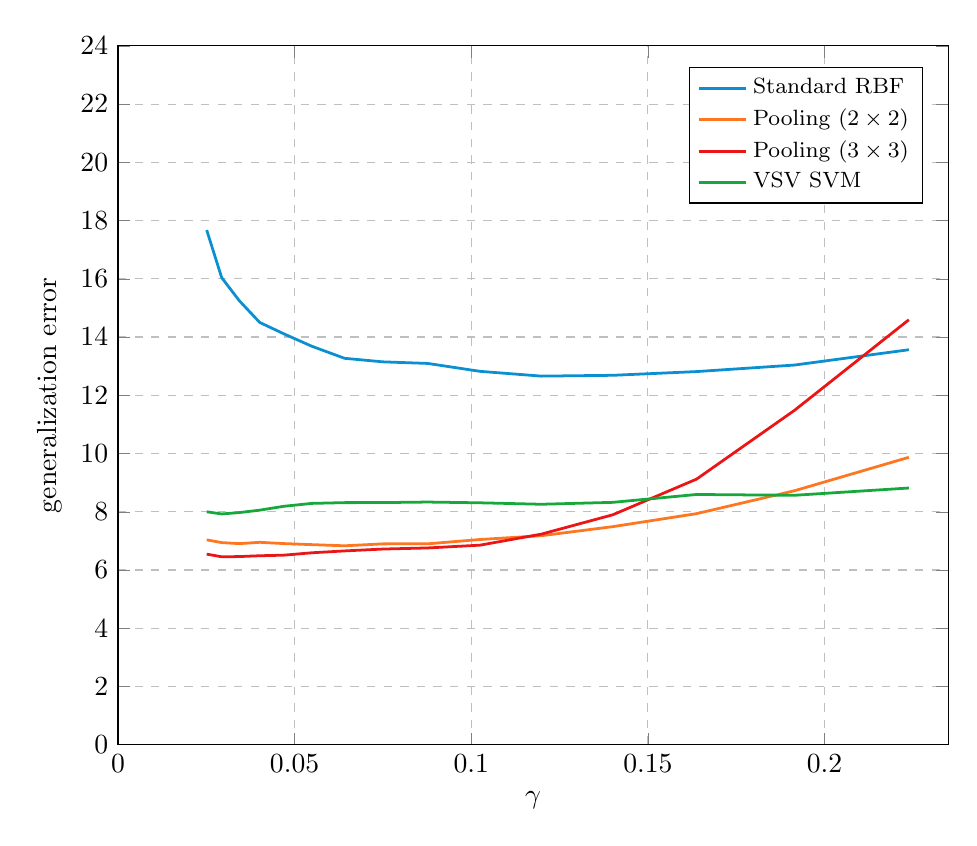
\begin{tikzpicture} \begin{axis}
[xmin=0, ymin=0, ymax=24, xmax=0.235, xlabel={$\gamma$}, ylabel={generalization error}, ymajorgrids=true, grid style=dashed, xmajorgrids=true, legend pos=north east, legend style={font=\footnotesize}, legend cell align={left}, xtick={0, 0.050, 0.10, 0.15, 0.20, 0.25}, ylabel near ticks, xlabel near ticks]

\legendentries

\addplot+[\RBF, no marks] coordinates {
(0.025118864315095794, 17.674)
(0.029366834982600287, 16.038)
(0.034333200182819934, 15.25)
(0.040139451033521366, 14.5)
(0.04692762459348836, 14.112)
(0.054863778484371045, 13.684000000000001)
(0.06414205312236927, 13.270000000000001)
(0.07498942093324558, 13.148)
(0.08767123872968682, 13.094)
(0.10249773907762157, 12.822)
(0.11983161944838325, 12.658000000000001)
(0.1400969148085072, 12.685999999999998)
(0.16378937069540642, 12.814000000000002)
(0.19148857053323368, 13.038)
(0.22387211385683395, 13.563999999999998)}; 

\addplot+[\Ptwo, no marks] coordinates {
(0.025118864315095794, 7.036)
(0.029366834982600287, 6.942)
(0.034333200182819934, 6.906000000000001)
(0.040139451033521366, 6.952)
(0.04692762459348836, 6.9079999999999995)
(0.054863778484371045, 6.872)
(0.06414205312236927, 6.832000000000001)
(0.07498942093324558, 6.898000000000001)
(0.08767123872968682, 6.9)
(0.10249773907762157, 7.048)
(0.11983161944838325, 7.178)
(0.1400969148085072, 7.49)
(0.16378937069540642, 7.936)
(0.19148857053323368, 8.722)
(0.22387211385683395, 9.87)}; 

\addplot+[\Pthree, no marks] coordinates {
(0.025118864315095794, 6.546000000000001)
(0.029366834982600287, 6.454000000000001)
(0.034333200182819934, 6.462000000000001)
(0.040139451033521366, 6.49)
(0.04692762459348836, 6.510000000000001)
(0.054863778484371045, 6.5920000000000005)
(0.06414205312236927, 6.656000000000001)
(0.07498942093324558, 6.720000000000001)
(0.08767123872968682, 6.758)
(0.10249773907762157, 6.854000000000001)
(0.11983161944838325, 7.232000000000001)
(0.1400969148085072, 7.897999999999999)
(0.16378937069540642, 9.122)
(0.19148857053323368, 11.482)
(0.22387211385683395, 14.594)}; 

\addplot+[\VSV, no marks] coordinates {
(0.025118864315095794, 8.0)
(0.029366834982600287, 7.925999999999999)
(0.034333200182819934, 7.9719999999999995)
(0.040139451033521366, 8.056000000000001)
(0.04692762459348836, 8.187999999999999)
(0.054863778484371045, 8.288)
(0.06414205312236927, 8.314)
(0.07498942093324558, 8.315999999999999)
(0.08767123872968682, 8.334)
(0.10249773907762157, 8.308000000000002)
(0.11983161944838325, 8.258)
(0.1400969148085072, 8.324)
(0.16378937069540642, 8.594)
(0.19148857053323368, 8.565999999999999)
(0.22387211385683395, 8.815999999999999)}; 

\end{axis} \end{tikzpicture} 

\caption{The 5-run averaged errors of a standard RBF SVM, two pooling SVMs and a VSV SVM on the artificial data set for various values of $\gamma$.} \label{fig:results1}
\end{figure}


%\begin{figure}[h!]
%\begin{center}
%\includegraphics[draft=false, width=1.0\columnwidth]{images/kernel-comparison.png}
%\end{center}
%\caption{The 5-run averaged errors of a standard RBF SVM, two pooling SVMs and a VSV SVM on the artificial data set for various values of $\gamma$.}
%\label{fig:results1}
%\end{figure}


\begin{table}[h!]
\centering
\caption{The minimum 5-run averaged errors of a standard RBF SVM, two pooling SVMs and a VSV SVM on the artificial data set with the corresponding $\gamma$ value.}
\label{tab:results1}
\begin{tabular*}{\columnwidth}{l@{\extracolsep{\fill}}rr} 
\toprule
SVM & min. average error & $\gamma$\\ 
\midrule 
Standard SVM & 12.66 & 0.120 \\
Pooling SVM ($2\times 2$) & 6.83 & 0.064 \\
Pooling SVM ($3 \times 3$) & 6.45 & 0.029\\ 
VSV SVM & 7.93 & 0.029\\ 
\bottomrule
\end{tabular*}
\end{table}


It is visible that the SVMs with pooling kernels as well as the VSV SVM have a lower generalization error than the classical RBF SVM for most values of $\gamma$. 
Clearly these three SVMs are more invariant against translations of the vertical lines, and can more often deduce the correct class than the standard SVM.
Further we see that the pooling SVMs perform slightly better than the VSV SVM, with an error of 6.83 and 6.45 for $2\times2$ and $3\times 3$ pooling respectively, versus 7.93 for the VSV method.
Thus, without enlarging the data set with manually defined transformations such as necessary for the VSV method, the pooling SVMs still manage to be more invariant than the VSV SVM and the standard RBF SVM. 

\subsection{Exp. 2: Pooling Kernels and Variable Training Set Sizes}

In the previous experiment the training set to test set ratio was 0.9, but what if we increased the number of training samples for each SVM?
Does each model perform equally well for a large number of training samples, or do the invariant SVMs have an edge over the standard SVM for this data set?
We performed a second experiment to determine the learning curves of the four SVMs for the same data set. 
Fig. \ref{fig:learningcurve} shows the learning curves of the four SVM models for training set sizes ranging from 5 to 1000, averaged over 5 runs.
For each SVM we used the corresponding $\gamma$ value in Table \ref{tab:results1} in each run. 

\begin{figure}[H] \centering
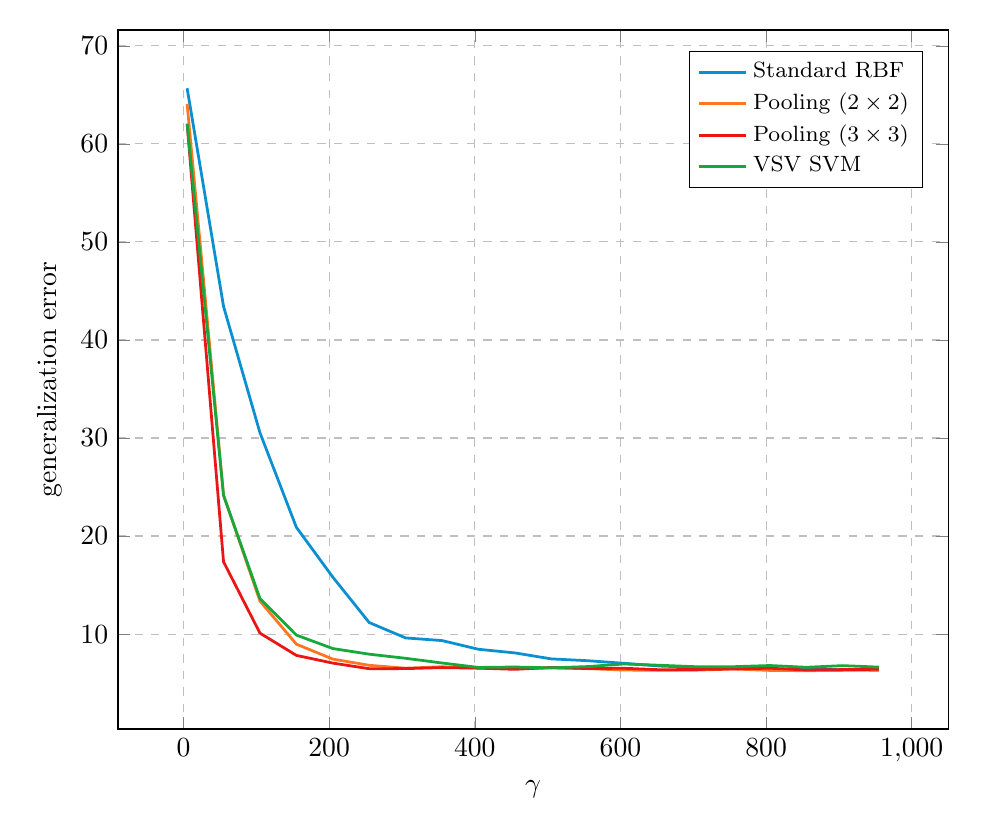
\begin{tikzpicture} \begin{axis}
[xlabel={$\gamma$}, ylabel={generalization error}, ymajorgrids=true, grid style=dashed, xmajorgrids=true, legend pos=north east, legend style={font=\footnotesize}, legend cell align={left}, xtick={0, 200, 400, 600, 800, 1000}, ylabel near ticks, xlabel near ticks]

\legendentries
\addplot+[\RBF, no marks] coordinates {
(5, 65.672)
(55, 43.42)
(105, 30.536)
(155, 20.892000000000003)
(205, 15.812000000000001)
(255, 11.178)
(305, 9.610000000000001)
(355, 9.34)
(405, 8.452000000000002)
(455, 8.081999999999999)
(505, 7.4719999999999995)
(555, 7.286)
(605, 7.019999999999999)
(655, 6.738000000000001)
(705, 6.606)
(755, 6.554)
(805, 6.42)
(855, 6.406000000000001)
(905, 6.369999999999999)
(955, 6.3100000000000005)}; 

\addplot+[\Ptwo, no marks] coordinates {
(5, 64.068)
(55, 24.188)
(105, 13.368)
(155, 8.974)
(205, 7.452)
(255, 6.8180000000000005)
(305, 6.5200000000000005)
(355, 6.67)
(405, 6.519999999999999)
(455, 6.4799999999999995)
(505, 6.542)
(555, 6.482000000000001)
(605, 6.33)
(655, 6.316000000000001)
(705, 6.324)
(755, 6.444)
(805, 6.295999999999999)
(855, 6.266)
(905, 6.299999999999999)
(955, 6.382)}; 

\addplot+[\Pthree, no marks] coordinates {
(5, 62.038)
(55, 17.372)
(105, 10.1)
(155, 7.83)
(205, 7.042)
(255, 6.469999999999999)
(305, 6.482000000000001)
(355, 6.581999999999999)
(405, 6.5280000000000005)
(455, 6.405999999999999)
(505, 6.598000000000001)
(555, 6.484)
(605, 6.516)
(655, 6.360000000000001)
(705, 6.396000000000001)
(755, 6.442)
(805, 6.522)
(855, 6.3420000000000005)
(905, 6.38)
(955, 6.409999999999999)}; 

\addplot+[\VSV, no marks] coordinates {
(5, 62.056000000000004)
(55, 24.136000000000003)
(105, 13.629999999999999)
(155, 9.898)
(205, 8.526)
(255, 7.952)
(305, 7.532000000000001)
(355, 7.052000000000001)
(405, 6.6)
(455, 6.642)
(505, 6.556)
(555, 6.688)
(605, 6.954000000000001)
(655, 6.8180000000000005)
(705, 6.668000000000001)
(755, 6.6739999999999995)
(805, 6.796000000000001)
(855, 6.614)
(905, 6.784000000000001)
(955, 6.632000000000001)}; 

\end{axis} \end{tikzpicture} 

\caption{Learning curves of a standard RBF SVM, two pooling SVMs and a VSV SVM on the artificial data set for fixed values of $\gamma$.} \label{fig:learningcurve}
\end{figure}

%\begin{figure}[h!]
%\begin{center}
%\includegraphics[width=1.0\columnwidth]{images/learning-curve.png}
%\end{center}
%\caption{Learning curves of a standard RBF SVM, two pooling SVMs and a VSV SVM on the artificial data set for fixed values of $\gamma$.}
%\label{fig:learningcurve}
%\end{figure}

Based on Fig. \ref{fig:learningcurve} we see that each classifier approaches the same performance as the number of training samples grows. 
Clearly classifier invariance is not necessary for this data set, as long as there are enough training samples. 
However, it is interesting to see that the invariant classifiers perform better when there are fewer training samples. 
We see that the pooling SVMs and the VSV SVM perform better than the standard SVM with training sets of fewer than 600 training samples. 
It is thus attractive to use invariant classifiers, if the number of training samples is limited. 
Further we see that the $2\times 2$ pooling SVM has a similar curve to the VSV SVM, but the $3\times 3$ pooling SVM performs even better than the other two in a small region.  
The lower errors of the $3\times 3$ pooling SVM can be explained by the larger range of transformations that are covered by the $3 \times 3$ pooling filter. 


\subsection{Exp. 3: Pooling SVMs and Noisy Data}


Max-pooling filters only extract the maximum values of the filter covered values, which means that max-pooling is mainly sensitive to the highest values in the input. 
If we consider a noisy input image, a max-pooling filter should be able to extract the original data from the image, as long as the noise values are small compared to the actual input values. 
Would a pooling SVM be able to perform better on a noisy data set than a standard SVM?

We investigated this by using the same artificial data set, to which positive Gaussian noise was added with a 0.2 standard deviation.
The values of the vertical lines are still higher than the noise values, so the max-pooling filter should be able to extract the vertical lines. 
Examples of the artificial data set with Gaussian noise are shown below. 


\begin{figure}[h!]
\begin{center}
\includegraphics[draft=false, width=0.95\columnwidth]{images/noise_lines.png}
\end{center}
\caption{Two samples of the noisy artificial data set with left a sample from class 1 and right a sample from class 2.}
\label{lines}
\end{figure}


\noindent

We recreated experiment 1 and experiment 2 using the noisy data set. 
Fig. \ref{fig:resultsnoise} presents the generalization error of the four SVMs on the noisy data set, averaged over 5 runs. 
Table \ref{tab:results2} shows the minimum error values of each SVM with the corresponding $\gamma$ value. 
Finally, we show the learning curves of the SVMs in Fig. \ref{fig:learningcurves2} using the $\gamma$ values in Table \ref{tab:results2} corresponding to each SVM.


\begin{figure}[H] \centering
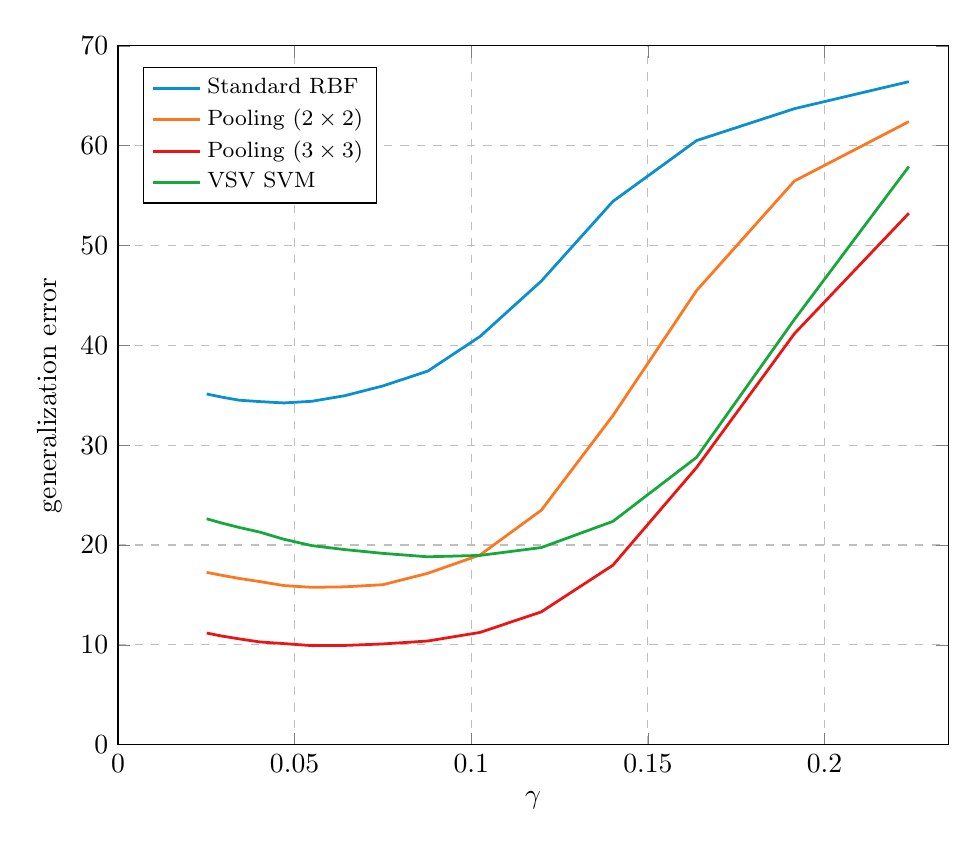
\begin{tikzpicture} \begin{axis}
[xmin=0, ymin=0, ymax=70, xmax=0.235, xlabel={$\gamma$}, ylabel={generalization error}, ymajorgrids=true, grid style=dashed, xmajorgrids=true, legend pos=north west, legend style={font=\footnotesize}, legend cell align={left}, xtick={0, 0.050, 0.10, 0.15, 0.20, 0.25}, ylabel near ticks, xlabel near ticks]

\legendentries
\addplot+[\RBF, no marks] coordinates {
(0.025118864315095794, 35.13)
(0.029366834982600287, 34.815999999999995)
(0.034333200182819934, 34.506)
(0.040139451033521366, 34.367999999999995)
(0.04692762459348836, 34.232000000000006)
(0.054863778484371045, 34.397999999999996)
(0.06414205312236927, 34.95399999999999)
(0.07498942093324558, 35.934)
(0.08767123872968682, 37.41799999999999)
(0.10249773907762157, 40.89)
(0.11983161944838325, 46.436)
(0.1400969148085072, 54.418000000000006)
(0.16378937069540642, 60.510000000000005)
(0.19148857053323368, 63.70399999999999)
(0.22387211385683395, 66.408)}; 

\addplot+[\Ptwo, no marks] coordinates {
(0.025118864315095794, 17.259999999999998)
(0.029366834982600287, 16.97)
(0.034333200182819934, 16.656)
(0.040139451033521366, 16.342)
(0.04692762459348836, 15.943999999999999)
(0.054863778484371045, 15.765999999999996)
(0.06414205312236927, 15.814000000000002)
(0.07498942093324558, 16.028)
(0.08767123872968682, 17.168)
(0.10249773907762157, 19.008000000000003)
(0.11983161944838325, 23.490000000000002)
(0.1400969148085072, 32.961999999999996)
(0.16378937069540642, 45.492)
(0.19148857053323368, 56.462)
(0.22387211385683395, 62.408)}; 

\addplot+[\Pthree, no marks] coordinates {
(0.025118864315095794, 11.186000000000002)
(0.029366834982600287, 10.888)
(0.034333200182819934, 10.602)
(0.040139451033521366, 10.295999999999998)
(0.04692762459348836, 10.13)
(0.054863778484371045, 9.925999999999998)
(0.06414205312236927, 9.943999999999999)
(0.07498942093324558, 10.094000000000001)
(0.08767123872968682, 10.388)
(0.10249773907762157, 11.25)
(0.11983161944838325, 13.307999999999998)
(0.1400969148085072, 17.98)
(0.16378937069540642, 27.77)
(0.19148857053323368, 41.176)
(0.22387211385683395, 53.23199999999999)}; 

\addplot+[\VSV, no marks] coordinates {
(0.025118864315095794, 22.628)
(0.029366834982600287, 22.204)
(0.034333200182819934, 21.759999999999998)
(0.040139451033521366, 21.296)
(0.04692762459348836, 20.582)
(0.054863778484371045, 19.944)
(0.06414205312236927, 19.548)
(0.07498942093324558, 19.165999999999997)
(0.08767123872968682, 18.824)
(0.10249773907762157, 18.962)
(0.11983161944838325, 19.747999999999998)
(0.1400969148085072, 22.369999999999997)
(0.16378937069540642, 28.786)
(0.19148857053323368, 42.6)
(0.22387211385683395, 57.906000000000006)}; 
\end{axis} \end{tikzpicture} 

\caption{The 5-run averaged errors of a standard RBF SVM, two pooling SVMs and a VSV SVM on the noisy artificial data set for various values of $\gamma$.} \label{fig:resultsnoise}
\end{figure}


%\begin{figure}[h!]
%\begin{center}
%\includegraphics[draft=false, width=1.0\columnwidth]{images/kernel-comparison-noise.png}
%\end{center}
%\caption{The 5-run averaged errors of a standard RBF SVM, two pooling SVMs and a VSV SVM on the noisy artificial data set for various values of $\gamma$.}
%\label{fig:resultsnoise}
%\end{figure}

\begin{table}[h!]
\centering
\caption{The minimum 5-run averaged errors of a standard RBF SVM, two pooling SVMs and a VSV SVM on the noisy artificial data set with the corresponding $\gamma$ value.}
\label{tab:results2}
\begin{tabular*}{\columnwidth}{l@{\extracolsep{\fill}}rr} 
\toprule
SVM & min. average error & $\gamma$\\ 
\midrule 
Standard RBF & 34.23 & 0.047 \\
Pooling SVM ($2\times 2$) & 15.77 & 0.055 \\
Pooling SVM ($3 \times 3$) & 9.93 & 0.055\\ 
VSV SVM & 18.82 & 0.088\\ 
\bottomrule
\end{tabular*}
\end{table}

\begin{figure}[H] \centering
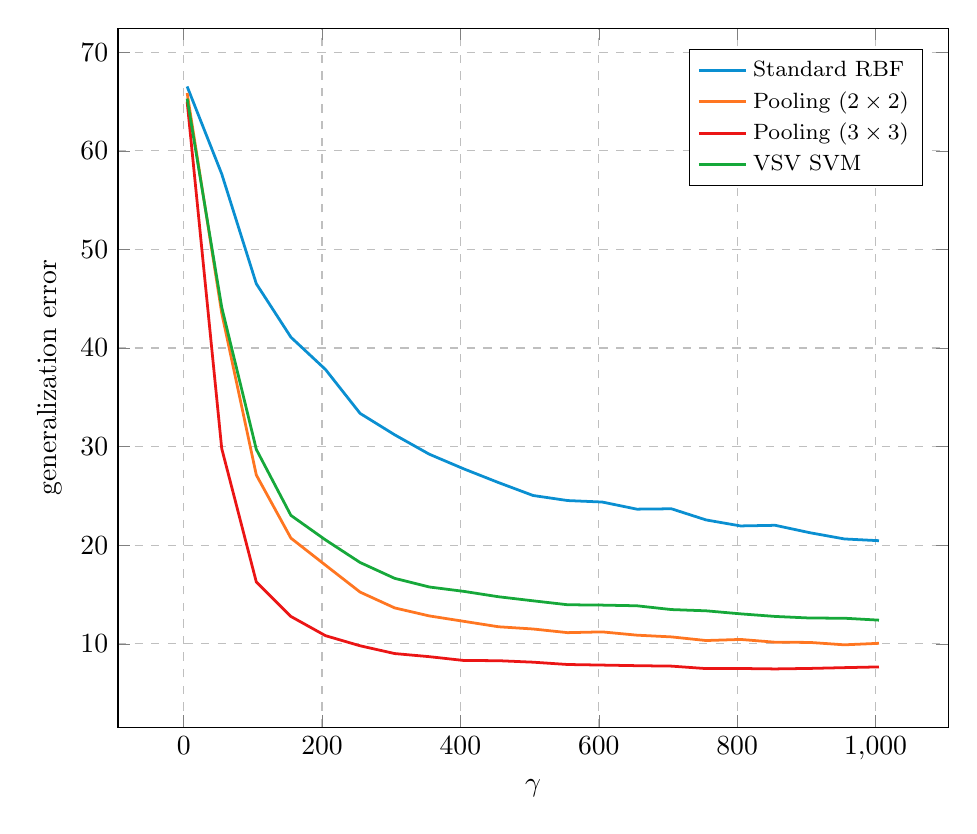
\begin{tikzpicture} \begin{axis}
[xlabel={$\gamma$}, ylabel={generalization error}, ymajorgrids=true, grid style=dashed, xmajorgrids=true, legend pos=north east, legend style={font=\footnotesize}, legend cell align={left}, xtick={0, 200, 400, 600, 800, 1000}, ylabel near ticks, xlabel near ticks]

\legendentries
\addplot+[\RBF, no marks] coordinates {
(5, 66.52799999999999)
(55, 57.653999999999996)
(105, 46.518)
(155, 41.096)
(205, 37.822)
(255, 33.370000000000005)
(305, 31.198)
(355, 29.232)
(405, 27.74)
(455, 26.356)
(505, 25.043999999999997)
(555, 24.53)
(605, 24.380000000000003)
(655, 23.657999999999998)
(705, 23.695999999999998)
(755, 22.566)
(805, 21.956)
(855, 22.020000000000003)
(905, 21.270000000000003)
(955, 20.636)
(1005, 20.458000000000002)}; 

\addplot+[\Ptwo, no marks] coordinates {
(5, 65.86800000000001)
(55, 43.547999999999995)
(105, 27.119999999999997)
(155, 20.720000000000002)
(205, 17.976)
(255, 15.246)
(305, 13.642)
(355, 12.829999999999998)
(405, 12.28)
(455, 11.73)
(505, 11.504)
(555, 11.132)
(605, 11.209999999999999)
(655, 10.878)
(705, 10.702000000000002)
(755, 10.334)
(805, 10.443999999999999)
(855, 10.162)
(905, 10.142)
(955, 9.898)
(1005, 10.052)}; 

\addplot+[\Pthree, no marks] coordinates {
(5, 64.99600000000001)
(55, 29.808)
(105, 16.27)
(155, 12.774000000000001)
(205, 10.826)
(255, 9.8)
(305, 9.012)
(355, 8.696)
(405, 8.309999999999999)
(455, 8.288)
(505, 8.138000000000002)
(555, 7.901999999999999)
(605, 7.843999999999999)
(655, 7.782000000000001)
(705, 7.7379999999999995)
(755, 7.4879999999999995)
(805, 7.498)
(855, 7.453999999999999)
(905, 7.504)
(955, 7.5840000000000005)
(1005, 7.6579999999999995)}; 

\addplot+[\VSV, no marks] coordinates {
(5, 65.30199999999999)
(55, 44.134)
(105, 29.718)
(155, 23.026)
(205, 20.538)
(255, 18.248)
(305, 16.639999999999997)
(355, 15.764)
(405, 15.318000000000001)
(455, 14.774000000000001)
(505, 14.362)
(555, 13.962)
(605, 13.925999999999998)
(655, 13.857999999999999)
(705, 13.474)
(755, 13.347999999999999)
(805, 13.039999999999997)
(855, 12.776)
(905, 12.616)
(955, 12.596)
(1005, 12.399999999999999)}; 

\end{axis} \end{tikzpicture} 

\caption{Learning curves of a standard RBF SVM, two pooling SVMs and a VSV SVM on the noisy artificial data set for fixed values of $\gamma$.}
\label{fig:learningcurves2}
\end{figure}


%\begin{figure}[h!]
%\begin{center}
%\includegraphics[draft=false, width=1.0\columnwidth]{images/learning-curve-noise.png}
%\end{center}
%\caption{Learning curves of a standard RBF SVM, two pooling SVMs and a VSV SVM on the noisy artificial data set for fixed values of $\gamma$.}
%\label{fig:learningcurves2}
%\end{figure}



\noindent
Fig. \ref{fig:resultsnoise} and Table \ref{tab:results2} clearly show that the pooling SVM has a better performance than the other SVMs. 
Not only does this hold for a small number of training samples, but also for larger training sets as suggested by Fig. \ref{fig:learningcurves2}.
For this particular data set we can say that the max-pooling filters make the SVMs more robust against noisy data.

%In Fig. \ref{fig:learningcurves2} we see similar bahavior as in Fig. \ref{fig:learningcurve}.
%The invariant SVMs perform better than the standard SVM for lower number of training samples. 
%Again, the pooling SVMs also perform better than the VSV SVM. 
%However, the difference between Fig. \ref{fig:learningcurve} and Fig. \ref{fig:learningcurves2} is that the four learning curves do not seem to converge to the same error values. 
%In contrast to the original data set, adding more training samples of the noisy data set does not make the standard SVM perform as well as the max-pooling SVMs. 
%For this particular data set, the max-pooling filters make the SVMs more robust against noisy data. 



%-------------------------------------------------------------------------



\section{Discussion}

{\color{lightgray}

Pooling worked in our case for simple input\\

Might not work for low resolution images as details are lost\\

Pooling helped against noise, but that means that pooling kernels are oblivious to certain textures, while they may be important\\

It is possible to combine multiple kernels with various filters\\





}


%-------------------------------------------------------------------------



{\small
\bibliographystyle{ieee_fullname}
\bibliography{egbib}
}

\end{document}

%-------------------------------------------------------------------------


%\begin{figure}[t]
%\begin{center}
%\fbox{\rule{0pt}{2in} \rule{0.9\linewidth}{0pt}}
%   %\includegraphics[width=0.8\linewidth]{egfigure.eps}
%\end{center}
%   \caption{Example of caption.  It is set in Roman so that mathematics
%   (always set in Roman: $B \sin A = A \sin B$) may be included without an
%   ugly clash.}
%\label{fig:long}
%\label{fig:onecol}
%\end{figure}



%\begin{figure*}
%\begin{center}
%\fbox{\rule{0pt}{2in} \rule{.9\linewidth}{0pt}}
%\end{center}
%   \caption{Example of a short caption, which should be centered.}
%\label{fig:short}
%\end{figure*}

